\documentclass[11pt]{article}
\usepackage[margin=1.2in]{geometry}
\usepackage{cite}
\usepackage{float}
\usepackage{tikz}
\usepackage{rotating}
\usepackage{lscape}
\usepackage{wrapfig}
\usepackage{pdflscape}
\usepackage{afterpage}

\usepackage{listings}
\lstloadlanguages{[Sharp]C}
\lstnewenvironment{code}
    {\lstset{}%
      \csname lst@SetFirstLabel\endcsname}
    {\csname lst@SaveFirstLabel\endcsname}
    \lstset{
      language=[Sharp]C,
      basicstyle=\small\ttfamily,
      flexiblecolumns=false,
      basewidth={0.5em,0.45em}
    }

\usetikzlibrary{shapes,arrows,positioning}

\tikzstyle{situation} = [rectangle, draw, fill=white!20, 
    text width=10em, text centered, minimum height=4em]
\tikzstyle{action} = [rectangle, draw, fill=white!20, 
    text width=8em, text centered, rounded corners=2em, minimum height=4em]
\tikzstyle{subsumptor} = [circle, draw, fill=white!20,
    text width=3em, text centered]
\tikzstyle{line_n} = [draw, -latex']
\tikzstyle{headless_n} = [draw]
\tikzstyle{anchor_n} = [inner sep=0pt, fill=none, draw=none]

\title{Team \(-i^2\)\\
AI For Games Coursework Submission (Tanks)}

\author{Connor Aspinall \and George Bell \and Denis Torgunov}

\date{}

\begin{document}

\maketitle
\begin{abstract}
  This report details the design and implementation of an AI player for a game of Tanks, based on a subsumptive architecutre. We highlight the improvements to our pathfinding module based on what we have learned during our work on the previous coursework, as well as detail our own implementation of subsumptive dispatch. We mention some of the issues we had during development and provide suggestions for future work and improvement.
\end{abstract}
\tableofcontents
\thispagestyle{empty}

\newpage

\section{Introduction}
This report details the implementation of a subsumption-based AI, as developed by the group ``Team \(-i^2\)''. The implemnetation focuses on an adaptive approcah and uses A* for effiecent pathfinding and navigation. It is meant to be extendible and the implementation produced, while succesful\footnote{was it?} during testing, was envisoned more as a proof of concept, with suggestions on better levereging the approach proposed given in section~\ref{sec:futureWork}.

Due to the fact that most of the codebase had to be implemented from scratch, as well as time constraints, the resulting AI might not be sufficiently optimised, and therefore unable to utilise CPU time provided in the most efficient manner. Suggestions for further optimisation are also given in section~\ref{sec:futureWork}.\footnote{Make sure that's true}

\section{AI Design and Implementation} \label{sec:design}

The AI produced by our group for this coursework focuses on utilising a subsumption architecture, inspired by the work done by one of the group members in the context of intelligent robotics. The subsumptive architecture, as proposed by Brooks, aims to form close connections between sensory inputs and behaviours of an intelligent agent\cite{brooks1}. In the context of an intelligent Tanks player, we can take information gleamed from the state of the map as simulating sensory inputs, and define a series of behaviours (such as running away, exploring, or seeking an enemy) to take in specific situtations. This approach lends itself well to group work, as individual components and behaviours can be developed separately, and then combined in arbitrairly complex ways using the subsumption architecture.

The binding of game situations (sensory inputs) to behaviours can be changed dynamically, or assigned at the start. For the purposes of this coursework, we define 2 major ``behavious profiles'' (as discussed in section~\ref{sec:behaviourProfiles}), a ``Hunter'' and an ``Explorer''. For the discussion of potential for dynamic and adaptive behaviour see section~\ref{sec:futureWork}.
\subsection{Subsumptive Control}

In order to make it possible to implement the subsumptive control system, we have created a class, \verb|SubsumptionDispatch|, which calls the corresponding action when the right ``stimulus'' occurs. For the full source code listing please see section~\ref{sec:subsumptionCode}. In this section we will only highlight the central parts of the implementation.

Firstly, we make use of C\# delegates to allow us to use higher-order methods, passing methods around as values and evoking them when needed. Specifically, we define the following two delegates:

\begin{code}
public delegate bool Situation();
public delegate ICommand Action();
\end{code}

A \verb|Situation| is a predicate that represents a situation in the game, corresponding to sensory input in a traditional subsumption architecture. An \verb|Action| represents a method that returns the next command to execute, corresponding to operating an acutator. It is assumed to take no arguments, relying purely on the internal state of the main class for any information about map composition, current player position, etc.

Having defined those delegates, we can create a dispatch table in a linked list of tuples:

\begin{code}
private List<Tuple<Situation, Action>> dispatchTable;
\end{code}

We assume that the first element in the list has the highest priority. If its \verb|Situation| arises, we execute the corresponding \verb|Action|. Otherwise, we continue down the list. We assume that at least one of the \verb|Situation|s will occur. In order to ensure that, the final element of the list should be a ``default'' action: simulated using a predicate that is always true.

With those definitons, we can now create the main program loop: the \verb|act()| method:

\begin{code}
public ICommand act()
{
  foreach (Tuple<Situation, Action> behaviour in dispatchTable)
  {
    if (behaviour.Item1())
    {
      return behaviour.Item2();
    }
  }
  return null;
}
\end{code}

As soon as the \verb|Action| whose \verb|Situation| predicate returns true is found, we simply execute that action, returning the corresponding command to be executed on this turn.

\subsection{Behaviour Profiles} \label{sec:behaviourProfiles}

We consider two possible behaviour profiles for is AI: the Hunter and the Explorer. The goal of the game it to maximise the score, and the behaviour process aims to do so in the most efficient way. If exploration is more valuable, point-wise, than killing opponents, we can utilise the Explorer profile, which focuses primarily on discovering the map and avoiding confrontation. On the other hand, if the amount of points received for killing an enemy is higher than the amount of points gained (on average) through exploration, we utilise the Hunter profile, which will actively seek to destroy enemy tanks.

Figure~\ref{fig:explorer} outlines the Explorer behaviour profile, and figure~\ref{fig:hunter} outlines Hunter. The Explorer aims to explore as much of the map as possible, while allowing the enemies to fight amongst themselves, only going on the offensive when there is a single enemy left. On the other hand, the Hunter actively seeks to gain points by destroying enemy tanks, and only then explores the remaining parts of the map.\footnote{refine the diagrams}

At present, we adopt the Explorer profile if the average score gain for discovering a rock or empty cell is larger than the score gain for destroying an enemy. This could be further improved, however appears to be a good ``ball-park'' metric.

\afterpage{
\clearpage
\begin{landscape}
\vspace*{\fill}
\begin{figure}[h]
  \centering
  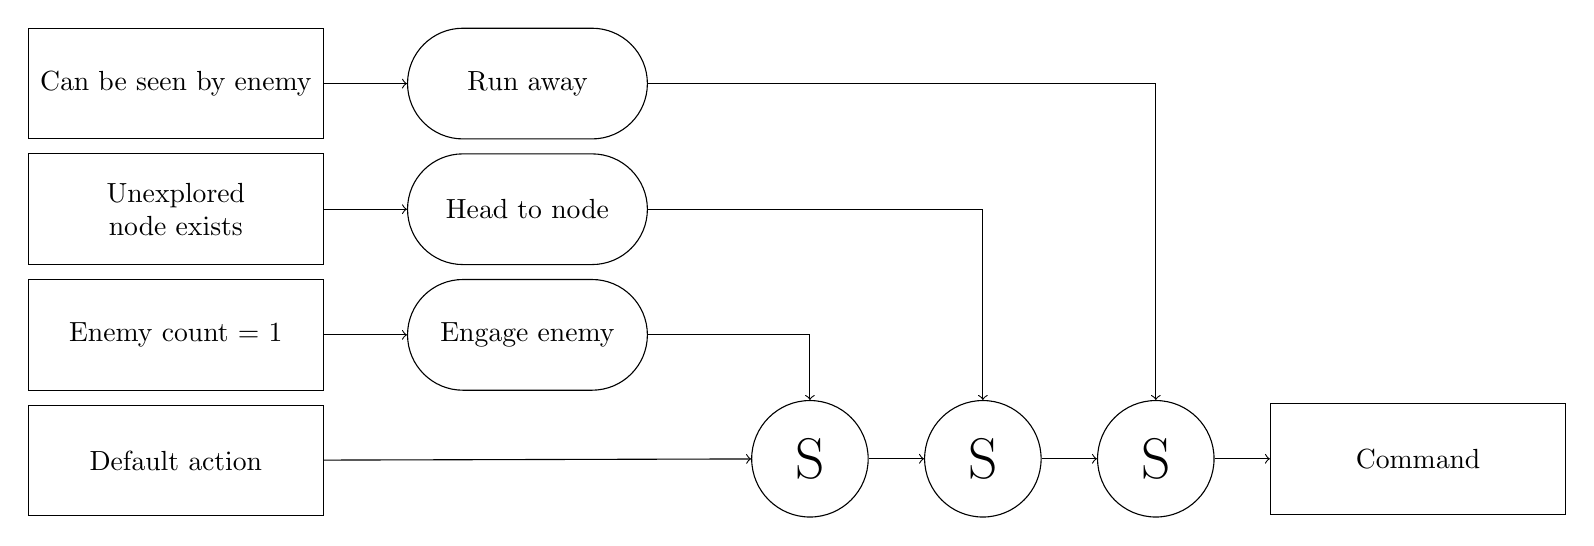
\begin{tikzpicture}[node distance=2cm, auto]
    \node[situation] (enemy) {Can be seen by enemy};
    \node[situation,below=0.5em of enemy] (unexploredNode) {Unexplored node exists};
    \node[situation,below=0.5em of unexploredNode] (singleEnemy) {Enemy count \(=\) 1};
    \node[situation,below=0.5em of singleEnemy] (default) {Default action};

    \node[action,right=3em of enemy] (runAway) {Run away};
    \node[action,right=3em of unexploredNode] (headTo) {Head to node};
    \node[action,right=3em of singleEnemy] (engage) {Engage enemy};

    \node[right=5.5em of engage] (anchorPoint) {};
    
    \node[subsumptor, below=2em of anchorPoint] (s1) {\huge S}; 
    \node[subsumptor, right=2em of s1] (s2) {\huge S}; 
    \node[subsumptor, right=2em of s2] (s3) {\huge S}; 
    
    \node[situation, right=2em of s3] (command) {Command};
    
    \path[draw,->] (default) -- (s1);
    \path[draw,->] (s1) -- (s2);
    \path[draw,->] (s2) -- (s3);
    \path[draw,->] (s3) -- (command);
    
    \path[draw,->] (enemy) -- (runAway);
    \path[draw,->] (unexploredNode) -- (headTo);
    \path[draw,->] (singleEnemy) -- (engage);
    
    \path[draw,->] (engage) -| (s1);
    \path[draw,->] (headTo) -| (s2);
    \path[draw,->] (runAway) -| (s3);
  \end{tikzpicture}
  \caption{The Explorer profile}
  \label{fig:explorer}
\end{figure}
\begin{figure}[h]
  \centering
  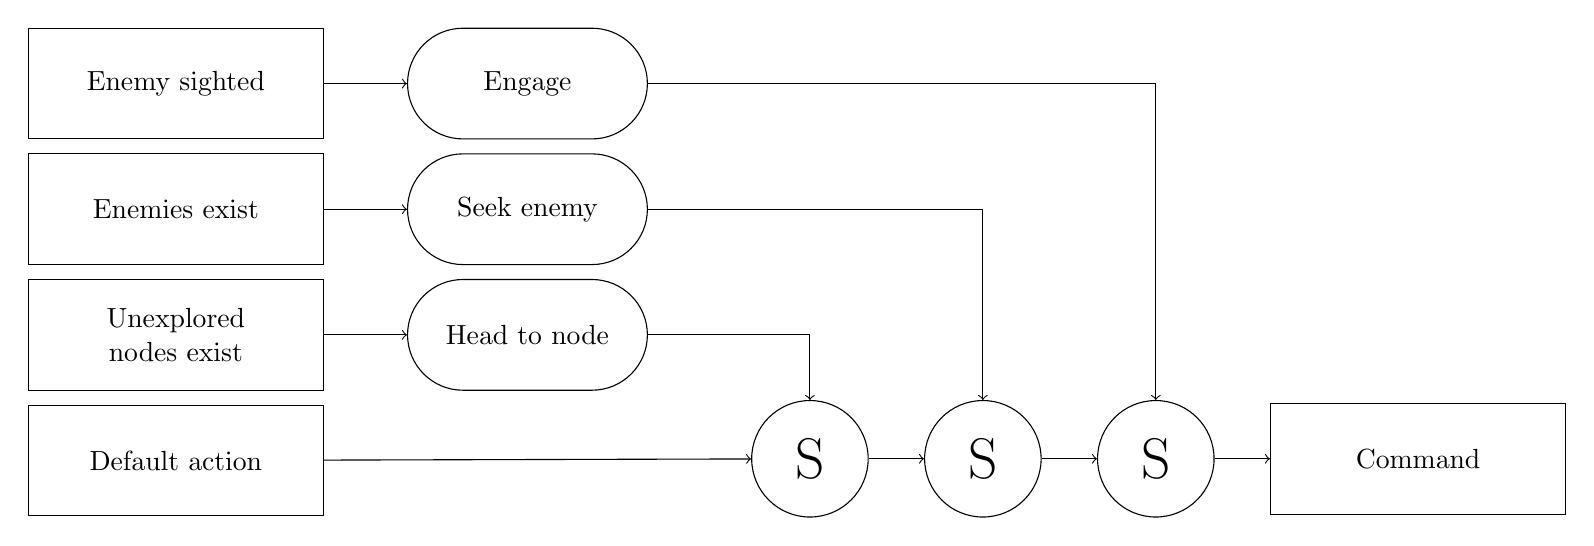
\begin{tikzpicture}[node distance=2cm, auto]
    \node[situation] (enemy) {Enemy sighted};
    \node[situation,below=0.5em of enemy] (unexploredNode) {Enemies exist};
    \node[situation,below=0.5em of unexploredNode] (singleEnemy) {Unexplored nodes exist};
    \node[situation,below=0.5em of singleEnemy] (default) {Default action};

    \node[action,right=3em of enemy] (runAway) {Engage};
    \node[action,right=3em of unexploredNode] (headTo) {Seek enemy};
    \node[action,right=3em of singleEnemy] (engage) {Head to node};

    \node[right=5.5em of engage] (anchorPoint) {};
    
    \node[subsumptor, below=2em of anchorPoint] (s1) {\huge S}; 
    \node[subsumptor, right=2em of s1] (s2) {\huge S}; 
    \node[subsumptor, right=2em of s2] (s3) {\huge S}; 
    
    \node[situation, right=2em of s3] (command) {Command};
    
    \path[draw,->] (default) -- (s1);
    \path[draw,->] (s1) -- (s2);
    \path[draw,->] (s2) -- (s3);
    \path[draw,->] (s3) -- (command);
    
    \path[draw,->] (enemy) -- (runAway);
    \path[draw,->] (unexploredNode) -- (headTo);
    \path[draw,->] (singleEnemy) -- (engage);
    
    \path[draw,->] (engage) -| (s1);
    \path[draw,->] (headTo) -| (s2);
    \path[draw,->] (runAway) -| (s3);
  \end{tikzpicture}
  \caption{The Hunter profile}
  \label{fig:hunter}
\end{figure}
\vspace*{\fill}
\end{landscape}
}

\subsection{Mapping and Pathfinding}

In order to make it easier to navigate and seek out enemies, we keep track not only of the visible area, but also of the overall map explored so far.  To that end, we have defined a \verb|Cell| enum. We keep and update an array of \verb|Cell|s, filling it with the ``visible'' information on each turn. 

We also keep track of the last place we saw enemy tanks, to make it easier to avoid or chase them later. This means that we also have to ``prune'' the map every so often, making sure there is at most one instance of each enemy (the one we saw most recently). For more details, please see section~\ref{sec:aiCode}.

The pathfinding algorithm we use is a refined and improved version of the A* implementation used in our previous coursework submission\cite{theGloriousWe}. We have cleaned up the \verb|GridNode| class, making it more streamlined, smaller and easier to use by removing redundant accessor functions. Since the class is only ever used within the project and no pre-processing of parameters is necessary, and no guarded conditions exist that could be expressed via setters, we simply made the relevant fields public. The only exception is \verb|GridNode.fCost|, which has been replacted with a getter that simply returns the relevant value based on the other parameters. This reduces the risk of \verb|GridNode.fCost| not being update properly by mistake.

In addition, we also have completely restructured the main pathfinding logic, in order to remove errors previously present. We have levereged what we have learned while implementing the first iteration\cite{theGloriousWe} and improved on the main shortcomings.

The most significant changes are as follows:

\begin{itemize}
\item Fixed an issue which caused the \verb|GridNode.fCost| be set inconsistantly while constructing the list of neighbours.
\item Fixed an issue where the path returned is not gaurenteed to be the shortest path as some \verb|GridNode|s where skipped unnecessarily.
\item Optimised the implementation by sorting the list to act as a priority queue, potentially reducing CPU time (depending on the native .NET sort implementation)
\item Made code more readable by using a stack when listing neighbours and looping through its contents instead of considering each neighbour explicitly when testing whether a coordinate is withing the bounds of the board array, as well as reducing complexity, as previously a nested loop was used
\end{itemize}

For the full listing of the pathfinding code please see section~\ref{sec:pathfindingCode}.

\subsection{Actions}

The actions that are carried out by the AI are dictated by the Subsumption Dispatch Table, which calls the relevant method in the class \verb|LocationLocator|, which attempts to find the best location to travel to in the given situation. This is achieved by having several methods, each relevant to one of the potental calls from the Subsumption Dispatch Table, with one being called each turn .

One of the key actions that can be carried out under the Explorer profile\footnote{Figure~\ref{fig:explorer}} is the run away action. This allows the AI to retreat when threated by an opponent, with the action being found in the \verb|Retreat| method of the \verb|LocationLocator| class. The full source code is listed in section ~\ref{sec:coward}. This method begins by generating a \verb|List| of \verb|GridNode|s found around the player that contain an obstacle that can be hidden behind. This list is initially generated from a 3-by-3 area which is centred on the player, however this are will be expanded if no suitable hiding locations are found. Due to the increasing complexity of this algorithm upon expansion\cite{GeorgeComplex}, it is capped at an area of 5-by-5, or an additional \verb|GridNode| in each direction. If, after analysing an area of that size and finding no suitable cover, it will default to dodging in a random direction until it moves closer to something it can take cover behind.

Upon finding a valid piece of cover, the AI will check behind it to see if it is a valid location.

\section{Testing and Tuning}

In order to test pathfinding and exploration without the oppontent AI destroying us, we have implemented a simple ``Useless'' AI, following the logic described in the lecture notes\footnote{Do we reeeeeeeeeeeally need a citation?}, that simply stays stationary and avoids attacking. This allowed us to safely navigate around the map and discover the bugs in the exploration part of the code\footnote{were they fixed?}.

In addition, problems arouse due to unexpected errors coming from Visual Studio. Firstly, we got errors trying to load the (standard) \verb|Tuple| class, so we have implemented our own, adhereing to the same naming conventions for elements, to make it interoperate with the code already written. Furthermore, more such errors appeared as more code was added. Eventually, we have decided to try changing the .NET framework version, and while that seemed to resolve the issue, it gave us cryptic warning that we did not have time to investigate in details and that might account for some of the bugs.

\section{Recommendations for Future Work} \label{sec:futureWork}

As mentioned earlier in section~\ref{sec:design}, it is possible to make this AI better by, instead of providing predefined behaviour profiles, allowing for a machine learning aspect by allowing the AI to learn, throughout the game, to associate specific \verb|Situation|s with the best \verb|Action|s, as well as adjusting the priority of each binding accordingly. Genetic programming might be a good fit for such a task. However, because it is impossible to save the information on the GridWorld servers themsevles between games, it means that the AI has to learn locally, which severely limits the applicability of this approach within the given setup.

The actions and predicates themselves could be further refined and optimised\footnote{George, please fill out as needed regarding the actions}.

Our approach to mapping and extracting infromation from the local map kept is, most likely, the least optimised part of the implementation. In particular, we have to loop through the whole array multiple times on each game loop iteration. Combining the tests performed into a single loop and making predicates simple accessors to the boolean fields holding the information gathered this way should make the code a lot more refined.

Finally, the pathfinding algorithm, as presented in the code, computes the path anew on each loop iteration. If the target cell has not changed, and there is no change in \verb|Situation|, it should be possible to cache the path initially computed, and simply continue moving as needed, greatly reducing the work done on each game loop iteration\footnote{Connor, please make sure this is right}.

\subsection{GridWorld Recommendations}
As mentioned above, the main element that we found missing in both this and the previous coursework submission for this module is the ability to retain information between runs on the GridWorld server. If each user was allocated a small amount of storage on the server, or a way to redirect some form of data to a text or binary file that could then be retrieved, it would be possible to view the server as a dynamic learning environment, broadening the applicability of machine learning approaches.
\section{Conclusions}

\newpage
% \clearpage
\addcontentsline{toc}{section}{References}
\bibliographystyle{IEEEtran}
\bibliography{IEEEabrv,references}

\newpage
\appendix

\section{Evidence of Group Work}
Throughout this project's development, Github has been used in order to synchronise our work and communicate issues. Below, we list the final log of git contributions, showing that all the group members have contributed. Note that, on average, people with less commits had more code added per commit.\footnote{Add git logs when done}
\section{Source code}
\end{document}